\documentclass[a4paper, notitlepage]{report}
\title{Smartphone Audio Acquisition and Synchronization Using an Acoustic Beacon}
\author{\sffamily\small S. Bosma, R. Smeding}
\date{}
% All imports needed for file

% General
\usepackage[a4paper,top=1.25in,right=1in,bottom=1.25in,left=1in]{geometry}
\usepackage[utf8]{inputenc}
\usepackage[T1]{fontenc}
\usepackage{textcomp}
\usepackage[bitstream-charter]{mathdesign}
\usepackage{cite}

\usepackage{import}
\usepackage{standalone}
\usepackage{epstopdf}



% Math
\usepackage{amsmath}	% some standard math functions
%\usepackage{amssymb}	% more mathematical symbols
\usepackage{amsbsy}	% enable bold mathematics
\usepackage{bm}
%\usepackage{amsthm}	% enable theorem statements
\usepackage{trfsigns} 	% symbols for transforms

% Text formatting
\usepackage{fancyhdr}	% allow more control over page headers/footers
\usepackage{enumitem}	% allow control over enumerate, itemize, description
\usepackage{setspace}	% allow control over spacing
\usepackage{lastpage}	% provide label for last page in document
\usepackage{sectsty}	% allow control over section styling
\usepackage{url}

% Floats
\usepackage{xcolor}		% enable use of colors
\usepackage{graphicx}		% enable graphics
\usepackage{float}		% enable floats
\usepackage[section]{placeins}	% prevent floats from moving past e.g. sections
\usepackage[small, bf, hang, figurename=Fig.]{caption}	% enable captions for floats (images etc.)
\captionsetup{width=.8\textwidth} % captions not too wide
\usepackage{subcaption}		% enable subcaptions for floats (images etc.)
\usepackage[nottoc]{tocbibind}		% put more stuff in TOC

% Styling data
\pagestyle{fancyplain}

% Title page
\makeatletter
\let\inserttitle\@title
\makeatother

% Page header
\setlength{\headwidth}{\textwidth}
\lhead{} % leave left header empty
\chead{}
\rhead{} % leave right header empty
\lfoot{} % leave left footer empty
\cfoot{} % leave center footer empty
\rfoot{}
\renewcommand{\headrulewidth}{0.3pt}
\renewcommand{\footrulewidth}{0pt}

% Section, equation and figure numbering
\usepackage{chngcntr} 
\counterwithout{figure}{chapter}
\renewcommand{\thechapter}{\Roman{chapter}}
\renewcommand{\thesection}{\Roman{chapter}.\arabic{section}}
\renewcommand{\thesubsection}{\Roman{chapter}.\arabic{section}.\arabic{subsection}}
\renewcommand{\thesubsubsection}{\alph{subsubsection})}
\renewcommand{\thefigure}{\arabic{figure}}
\renewcommand{\thesubfigure}{\alph{subfigure}}
\renewcommand{\theequation}{\thechapter--\arabic{equation}}
\setcounter{tocdepth}{1}
\captionsetup[figure]{labelsep=period}

% Nice enumerations
\newlist{enum}{enumerate}{1}
\setlist[enum]{label=\textbf{[\arabic*]}} % \arabic or \alpha
\setlist{itemsep=-5pt}

% Nice \begin{StateDescription} for FSM descriptions
\newlist{StateDescription}{description}{1}
\setlist[StateDescription]{font=\normalfont\scshape, labelwidth=12em, leftmargin=12em,listparindent=0em,itemindent=0em}

% Section formatting
\definecolor{title-gray}{gray}{0.45}		% grijstint voor headers
\renewcommand*\sfdefault{lmss}
\allsectionsfont{\sffamily\color{title-gray}}	% sans-serif in headers

% Page layout
\onehalfspacing					% Wide margins for text
\usepackage{chngpage}			% customize margins of certain pages
\usepackage{adjustbox}

% Text macros
\usepackage{xspace}
\newcommand{\matlab}{MATLAB\xspace}		% fancy MATLAB command
\newcommand{\norm}[1]{\left\lVert#1\right\rVert}% Command for vector norm
\newcommand{\abs}[1]{\left\lvert#1\right\rvert}% Command for abs
\newcommand{\todo}[1]{\textbf{\textcolor{red}{#1}}}	% placeholder stuff
\let\oldhat\hat
\renewcommand{\vec}[1]{\bm{#1}} % bold vectors in math mode
\newcommand{\vechat}[1]{\oldhat{\bm{#1}}} % hat in vector mode
\newcommand{\mat}[1]{\bm{#1}} % bold matrix in math mode

%links
\usepackage{hyperref}
\hypersetup{ %setup hyperlinks
    colorlinks=true,
    citecolor=black,
    filecolor=black,
    linkcolor=black,
    urlcolor=black
}

\begin{document}

\section{MATLAB implementation}
\label{sec:matlab}
The possibility to call compiled Java \texttt{.class} files from within \matlab can be used to leverage Java's asynchronous networking capabilities from within a \matlab script. In this section, the implemented Java/\matlab host application will be detailed and design choices will be explained.

\paragraph*{}
The choice for \matlab was made based on the ease of prototyping, prior experience and interconnections with the subsystem built by van Wijngaarden and Wouters \cite{BAP:ErikNiels}. Furthermore, compiled Java \texttt{.class} files can be called from \matlab to extend default \matlab functionality.

\paragraph*{}
Although \matlab was found to provide a suitable environment for developing this application, it was found that interoperation between Java code and \matlab itself is not entirely trivial. The largest problem is that the ability to call back arbitrary \matlab functions from Java, while present, is not officially supported or documented\footnote{Yair Altman keeps a blog called Undocumented Matlab where he explains how \matlab callbacks can be implemented in Java, among other undocumented features: \url{http://www.undocumentedmatlab.com}}. Using this functionality is therefore somewhat risky, since MathWorks may remove this functionality without any indication to users.

\paragraph*{}
Despite previously mentioned concerns, it was decided to use Java for this project because \matlab does not natively provide non-blocking networking to multiple clients. In Java, the \texttt{java.nio} package developed by Oracle\footnote{Documentation for the NIO package can be found at \\ \url{https://docs.oracle.com/javase/7/docs/api/java/nio/package-summary.html}} allows multiple simultaneous transmission control protocol (TCP) connections over a single port, enabling multiple smartphones to connect to the Java program. The connections can then be multiplexed using \texttt{selector}. The reason TCP was chosen instead of the user datagram protocol (UDP) is the connection-oriented nature of TCP, which provides guaranteed in-order reception of packets. This simplifies consequent signal processing, which no longer has to account for possibly missing audio data.

\paragraph*{}
Using a single processing thread would cripple this server application since the application could then either send/receive data to connected clients \emph{or} process the received audio. In order to parallelize these concurrent activities, the Java classes utilized parallelization in the form of \texttt{java.lang.Thread} threads. One thread is used to perform non-blocking I/O and the other thread is the default \matlab thread used to process incoming audio samples.

\subsection{I/O finite state machine}
\label{sec:io_fsm}
Since the I/O is non-blocking, several clients (in this case, smartphones) can read and write to the server simultaneously. Therefore, to facilitate communicating with multiple devices simultaneously, the server application represents each client as a finite state machine (FSM). From the server's point of view, each client is in one of the following states (see also Fig.~\ref{fig:fsm-server}):

\begin{StateDescription}
\item[configuring] The client has initiated a connection to the server and the client and server are currently negotiating settings\footnote{The negotiated settings are sample rate, block length (number of bytes sent at once) and mono/stereo recording.}.

\item[idle] The client is connected and fully configured. It is awaiting a start streaming command to start streaming its audio recordings to the server. Additionally, the settings may be renegotiated to change the state back to \textsc{configuring}.

\item[streaming] The client is currently streaming audio to the server. Sending a stop streaming signal will change the client state to \textsc{idle}.
\end{StateDescription}
\noindent
Additionally, because a complete packet sent by a client may arrive as several frames on the server side, each client can be in one of two reading states:
\begin{StateDescription}
\item[receivingdata] This state indicates to the server that the client is somewhere along sending a packet to the server. The next read frame should be interpreted as a continuation of the previous frame(s).
\item[idle] This state indicates the next received frame should be interpreted as the start of a new packet.
\end{StateDescription}

\begin{figure}[htb]
\centering
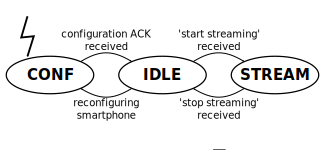
\includegraphics[width=0.8\textwidth]{figures/implementation/server_fsm}
\caption[Server and Android app FSM.]{Diagram representing the finite state machine implemented by both the server and the smartphone application.}
\label{fig:fsm-server}
\end{figure}

\subsection{Communication protocol}
\label{subsec:communication-protocol}
On top of the TCP interface provided by the Java \texttt{SocketChannel}\footnote{Documentation for the SocketChannel can be found at \url{https://docs.oracle.com/javase/7/docs/api/java/nio/channels/SocketChannel.html}}, a custom communication protocol between the \matlab application and the clients was defined. Each packet starts with one byte identifying its type to the recipient. A list of each byte-identifier and packet type in the communication link along with their content is listed below.
\begin{StateDescription}
\item[1: setup] Sent from server to client. Contains 4 bytes specifying the sampling rate to use, 4 bytes containing the block length to use and 1 byte indicating whether to record in mono or stereo.

\item[2: ack\_setup] Sent from client to server after receiving \textsc{setup}. Contains a string with the hardware (MAC) address of the client preceded by 4 bytes specifying, in bytes, the length of the string.

\item[3: start\_streaming] Sent from the server to the client, indicating the client should start streaming its audio recordings to the server. Contains 1 byte specifying which audio source to use, as explained in section \ref{sec:android}.

\item[4: stop\_streaming] Sent from the server to the client, indicating the client should cease streaming its audio recordings to the server. Packet has no content.

\item[5: ack\_stop] Sent from the client to the server to acknowledge it has received the stop packet and will stop streaming audio. Packet has no content.

\item[6: stream\_data] Sent from client to server, contains recorded audio samples. The length of this packet is $\text{block\_length}*16~ \text{bits}$ (each sample has 16 bit resolution). The block length is negotiated in the \textsc{setup} packet.

\item[7: orientation\_update] Sent from client to server, contains 12 bytes (3 floating point numbers) with measured azimuth, pitch and roll. A final byte indicates whether the phone is moving\footnote{This byte is not used on the \matlab side.}. 
\end{StateDescription}

\end{document}
